\section{Image Segmentation}
\subsection*{Complete segmentation}
Finite set of non-overlapping regions that cover the whole image $I = \bigcup_{i = 1}^{n} R_i$ and $R_i \cap R_j = \emptyset$ $\forall i, j, i \neq j$\\
\greenbf{Thresholding:} simple segmentation by comparing greylevel with a threshold to decide if in or out.\\
\greenbf{Chromakeying:} when planning to segment, use special backgroundcolor. (Problems variations due to lighting, noise, halo around foreground due to aliasing mixed pixels due to motion blur(hard $\alpha$-mask does not work)) $I_\alpha = |I - g| > T$
\subsection*{Receiver Operating Characteristic (ROC) analysis:}
ROC curve characterizes performance of binary classifier Classification errors: False negative (FN), false positives (FP)\\
ROC curve plots TP fraction $\frac{TP}{TP + FN}$ vs FP fraction $\frac{FP}{FP + TN}$\\
\greenbf{Operating points:} choose point with gradient
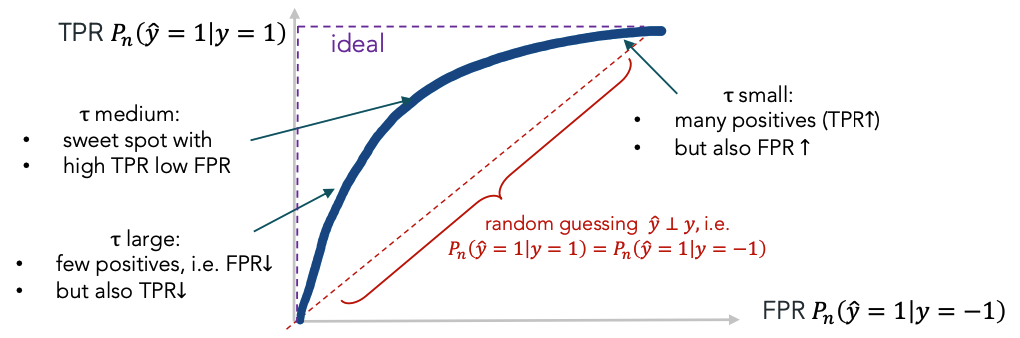
\includegraphics[width=0.4\columnwidth]{jo/roc.png} 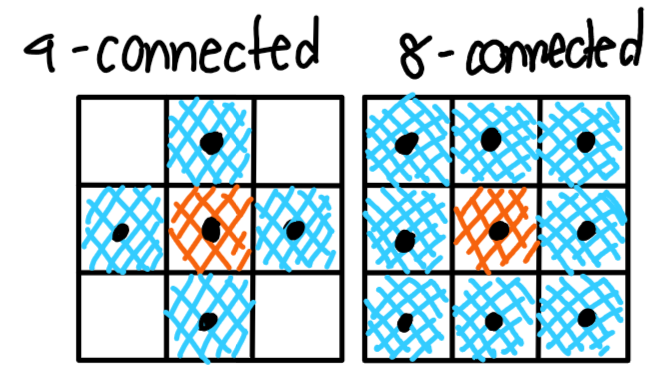
\includegraphics[width=0.4\columnwidth]{jo/connection.png}
\subsection*{Pixel connectivity}
\graytext{also regions if $x$-connected}\\
\greenbf{Connected component raster scanning:} scanning row by row, if foreground \& label if connected to other label, else give new label. (second pass to find equivalent labels)\\
\greenbf{Improve:} when region found, follow border, then carry on (contour-based method)
\subsection*{Region growing}
Start with seed point or region, add neighboring pixels that satisfy a criteria defining a region until we include no more pixels.\\
\greenbf{Seed region:} by hand or automatically by conservative Thresholding\\
\greenbf{Inclusion criteria:} greylevel thresholding, greylevel distribution model (include if ($I(x, y) - \mu^{2})^{2} < (n \sigma)^{2}$ and update $\mu$ and $\sigma$ after each iteration) color or texture information\\
\greenbf{Snakes:} active contour, a polygon and each point moves away from seed while criteria is met (can have smoothness constraint) Iteratively minimize enery function $E = E_{tension} + E_{stiffness} + E_{image}$
\subsection*{Background subtraction}
simple: $I_\alpha = |I - I_{bg}| < T$ better: $I_\alpha = \sqrt{(I - I_{bg})^T \Sigma^{-1} (I - I_{bg})}$ where $\Sigma$ is the background pixel appearance covariance matrix, computed seperately for each pixel. (Mahalanobis Distance uses mean instead of $I_{bg}$)
\subsection*{Morphological operators}
Logical transformations based on comparison of neighboring pixels. Inputs: Binary image, structuring element $S$. \\
\greenbf{Erode: } $E = \{x:x+s \in I, $for every $ s \in S\}$\\
\graytext{delete FG pixels with 8-connected BG pixels} \\
\greenbf{Dilate: }  $E = \{x:x-s, y \in I $ and $ s \in S\}$\\
\graytext{every BG pixels with 8-connected FG pixel make a FG pixel}\\
\greenbf{Opening:} $(I \ominus S) \oplus S$ \quad
\greenbf{Closing:} $(I \oplus S) \ominus S$\\
\greenbf{Uses:} smooth regions, remove noise and artifacts.